\begin{figure}[h!]
    \centering
    \begin{subfigure}[c]{0.48\linewidth}
        \centering
        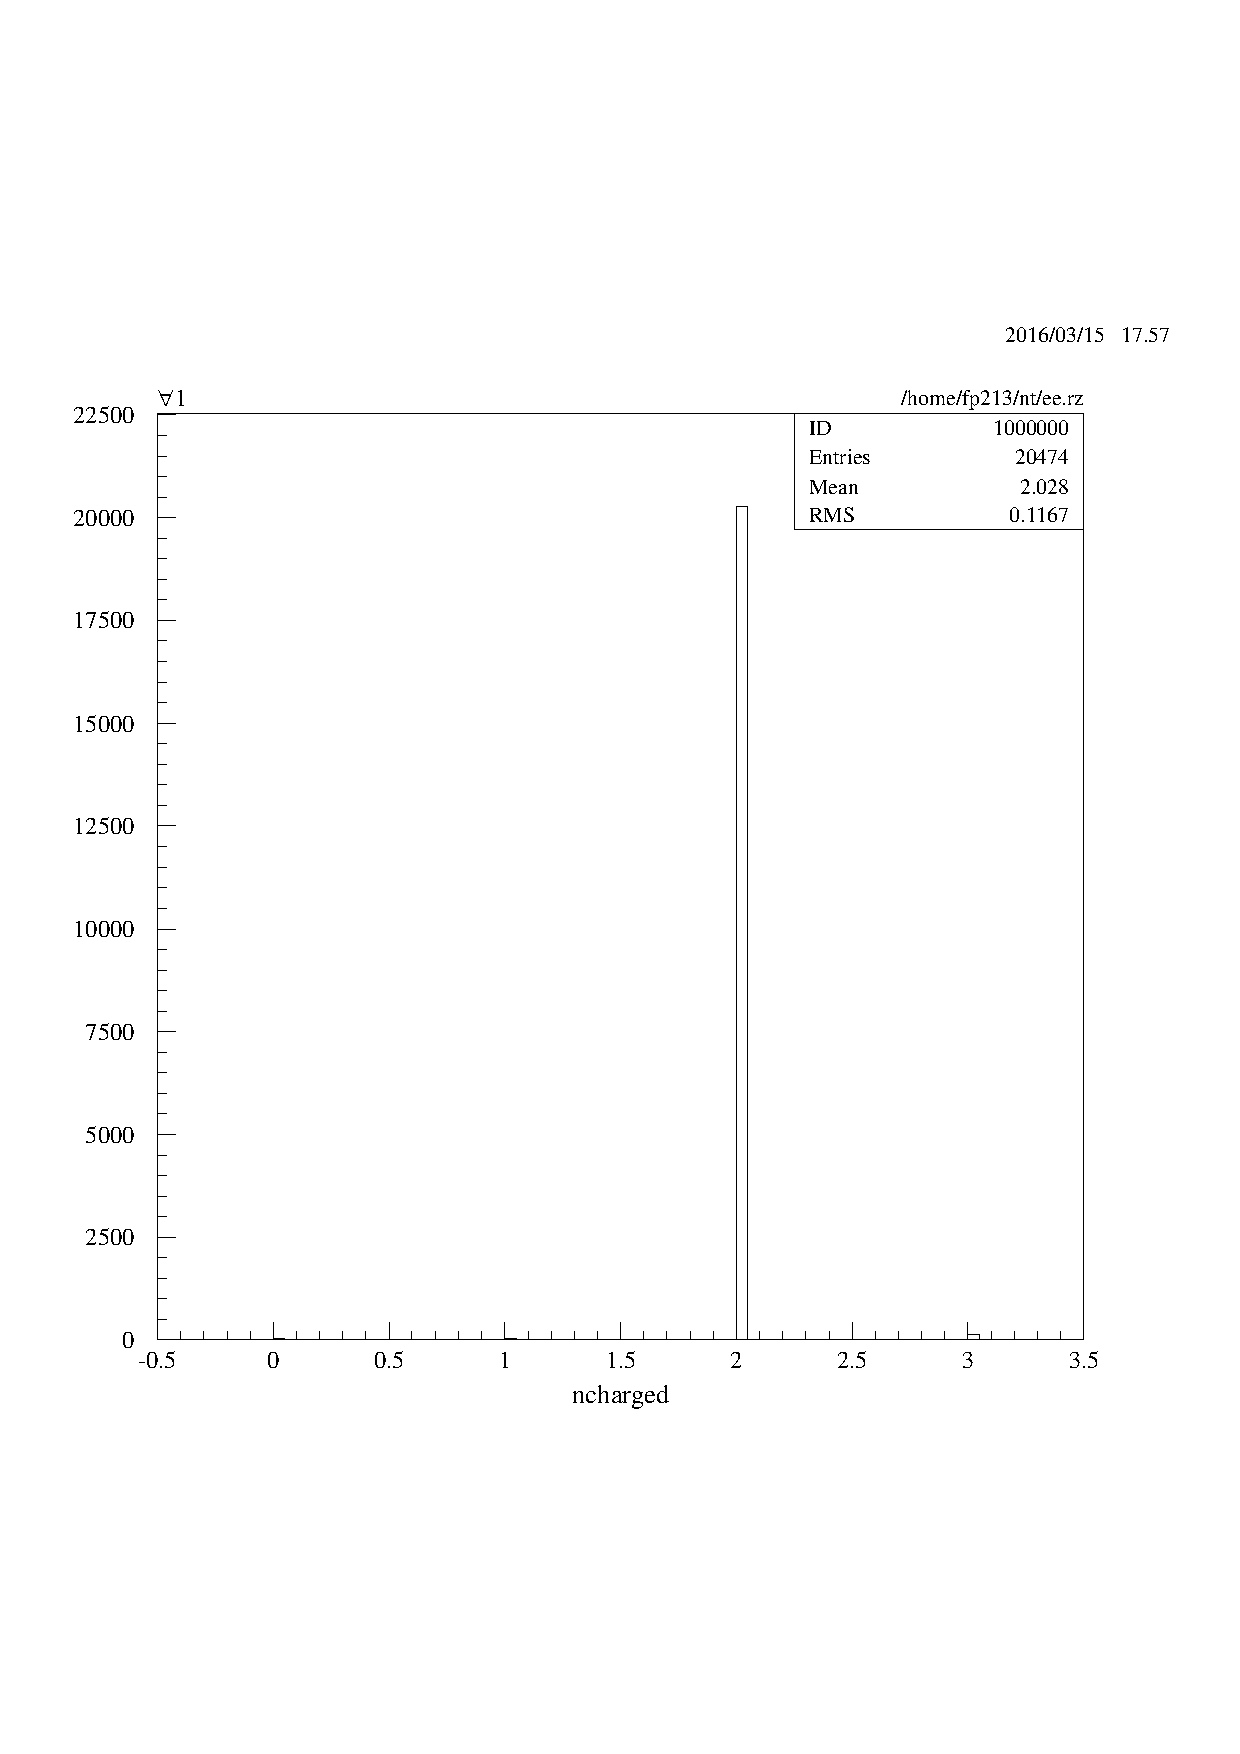
\includegraphics[width=\linewidth]{matrix-electrons-with-electron-filter}
        \caption{%
            Electrons with electron cut
        }
        \label{fig:paw-matrix/electrons}
    \end{subfigure}
    \hfill
    \begin{subfigure}[c]{0.48\linewidth}
        \centering
        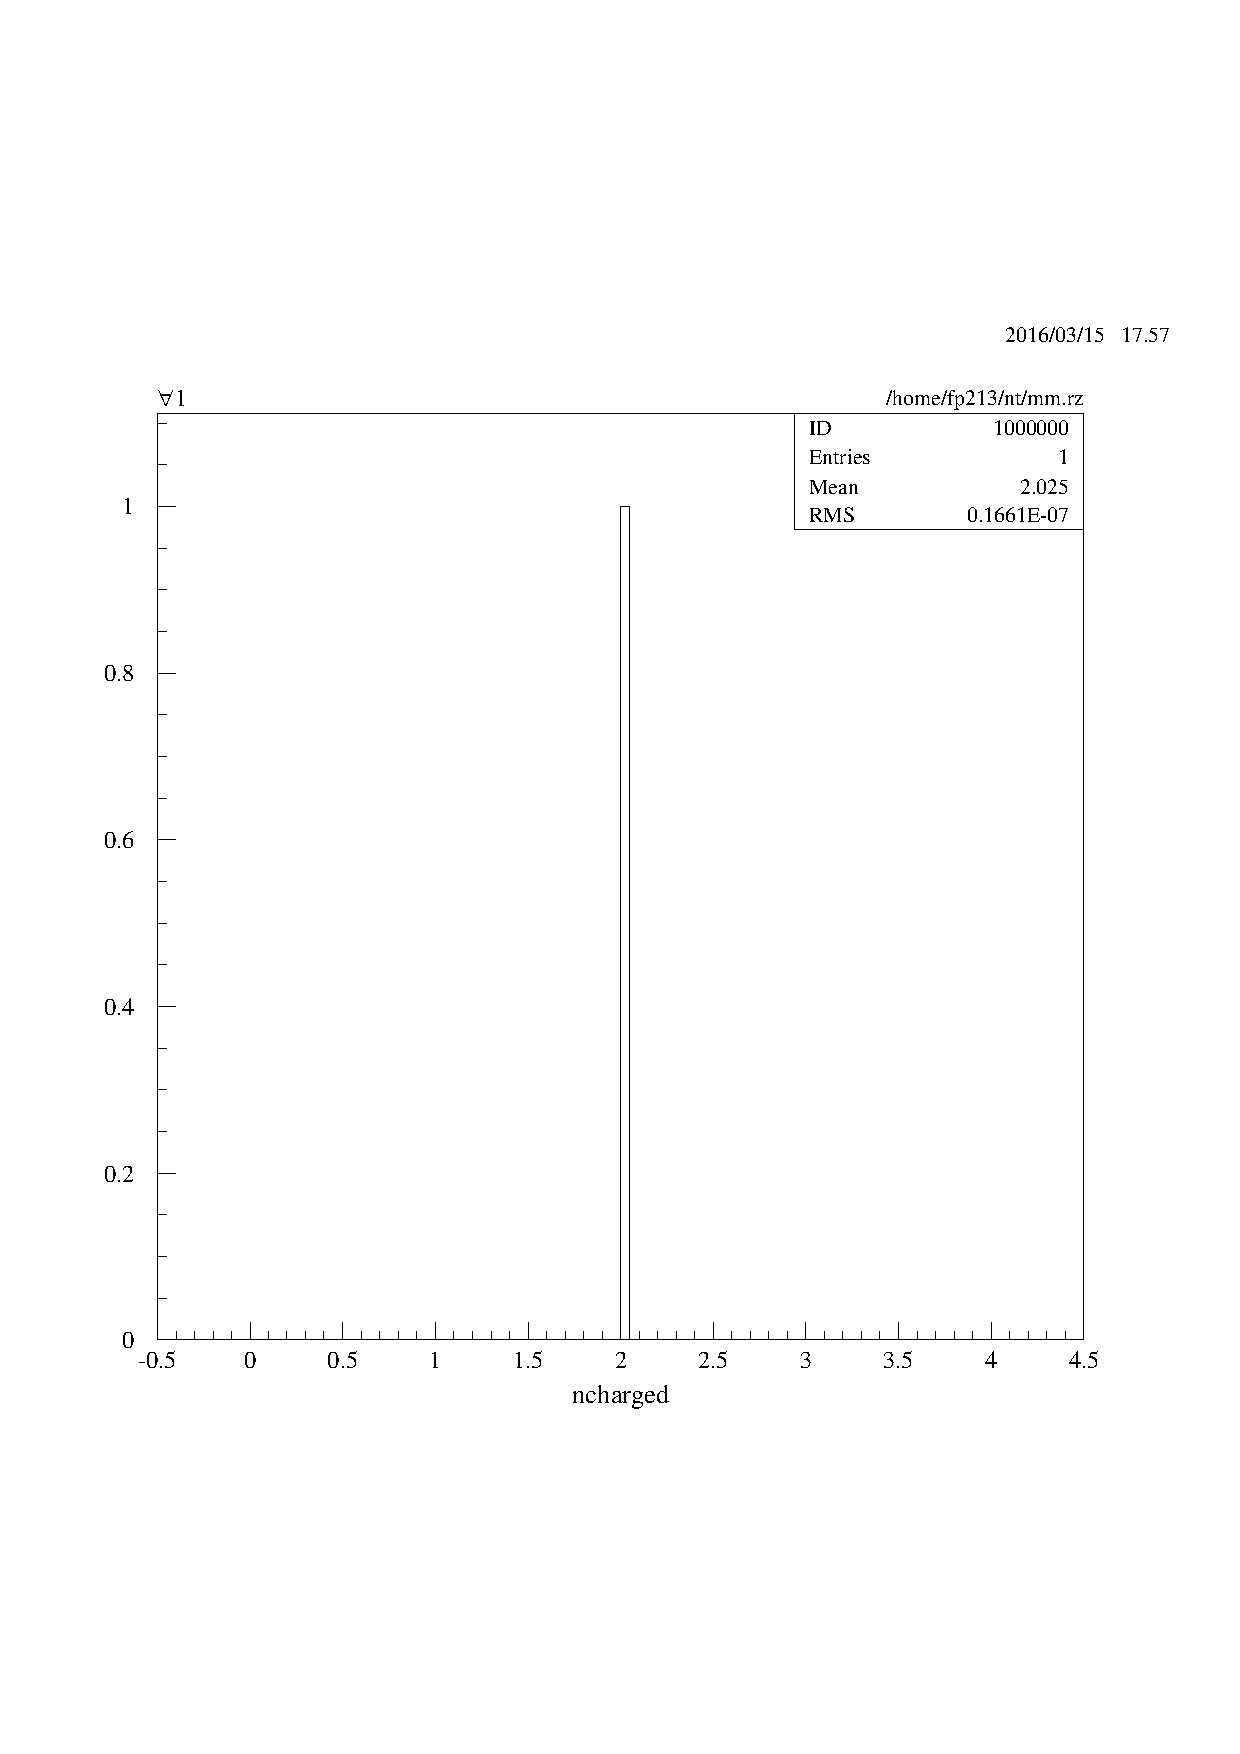
\includegraphics[width=\linewidth]{matrix-muons-with-electron-filter}
        \caption{%
            Muons with electron cut
        }
        \label{fig:paw-matrix/muons}
    \end{subfigure}
    \caption{%
        Histograms to obtain number of matched events in out cuts. Created with
        \textsc{paw} from Monte Carlo datasets.
    }
    \label{fig:paw-matrix-electrons}
\end{figure}
